\documentclass{article}

\usepackage{tikz}
\usepackage{pgfplots}
\usetikzlibrary{patterns, backgrounds}

\title{Setting Up an ETB Network}
\author{Gr\'egoire Hamon}
\author{Ian Mason}

\long\def\omitthis#1{\relax}

\begin{document}

\maketitle

\section{Introduction}

An ETB network is composed of one or several connected ETB servers.
This network is fully connected: any server can contact any other
server directly. An ETB network can also link another ETB network
through a gateway. In this case any communication with the linked
network is done through the gateway, the linked network does not have
any knowledge of the contacting ETB network.

\section{Connected Server}

\subsection{The {\tt connect} Method}

A source ETB server can be asked to connect to a destination ETB
server using the {\tt connect} XML-RPC method:
\begin{verbatim}
connect(host, port)
\end{verbatim}
Once the connection is established, both the source and destination
propagate the information about the new server to their respective ETB
network, practically merging the two ETB networks once the propagation
is complete.

\tikzstyle{server}=[circle,draw,inner sep=0pt,minimum size=10mm, node distance=20mm]

\begin{figure}[h]
\begin{tikzpicture}[thick]
  \node[server] (A) {A} ;
  \node[server] (B) [below of=A] {B}
    edge(A);
  \node[server] (C) [right of=A] {C};
  \node[server] (D) [below of=C] {D}
    edge(C);

  \draw [->] (3.5,-1)--(5.5,-1) node [above,midway] { A.connect(C) };

 \begin{scope}[xshift=7cm]
   \node[server] (A') {A};
   \node[server] (B') [below of=A'] {B}
     edge(A');
   \node[server] (C') [right of=A'] {C}
     edge(A')
     edge(B');
   \node[server] (D') [below of=C'] {D}
     edge(A')
     edge(B')
     edge(C');
 \end{scope}
\end{tikzpicture}
\caption{Connecting Two ETB Networks}
\label{fig:connect}
\end{figure}
Figure~\ref{fig:connect} shows two ETB networks, with two servers
each, and the results of calling the {\tt connect} method of the
server {\tt A}, with the address and port of the server {\tt C}. The
resulting network contains all the servers of both networks and is
fully connected.

\subsection{Connecting a server in etb-shell}

In the etb-shell, the {\tt connect} command has exactly the same
signature as the {\tt connect} method. For example, assuming that the
etb-shell is connected to an ETB server, the command:
\begin{verbatim}
> connect(localhost, 24567)
\end{verbatim}
Calls the {\tt connect} method of the server with the arguments {\tt
  localhost} and {\tt 24567}.

\omitthis{
\section{Linked Server}

\subsection{The {\tt link} Method}

Connected servers are the normal way to establish an ETB network.
There are situation where such connection are not possible or
desirable. For example if the servers are on separate networks, it is
not always possible to get the full connectivity required by the ETB.

In such cases, ETB networks can be linked. In this mode of connection
two ETB networks communicate through a gateway server on each network.
Links have a direction: the source ETB network uses the destination
network to process queries,

An ETB server exposes a {\tt link} XML-RPC method:
\begin{verbatim}
link(host, port, my_port=NULL)
\end{verbatim}
The arguments {\tt host} and {\tt port} are the host and the port to
link to. The optional argument is used to overwrite the ETB server's
default port. It is used when communication has to go through a tunnel
-- see section~\ref{sec:using-links-connect} for details.

\begin{figure}[h]
\begin{tikzpicture}[thick]
  \node[server] (A) {A} ;
  \node[server] (B) [below of=A] {B}
    edge(A);
  \node[server] (C) [right of=A] {C};
  \node[server] (D) [below of=C] {D}
    edge(C);

  \draw [->] (3.5,-1)--(5.5,-1) node [above,midway] { A.link(C) };

 \begin{scope}[xshift=7cm]
   \node[server] (A') {A};
   \node[server] (B') [below of=A'] {B}
     edge(A');
   \node[server] (C') [right of=A'] {C}
     edge [<-,dashed] (A');
   \node[server] (D') [below of=C'] {D}
     edge(C');
 \end{scope}
\end{tikzpicture}
\caption{Connecting Two ETB Networks}
\label{fig:link}
\end{figure}
Figure~\ref{fig:link} shows the effect of linking two example ETB
networks. The server {\tt B} can use resources of the server {\tt D},
but any request is routed through the servers {\tt A} then {\tt C}.
The server {\tt C} and {\tt D} cannot use resources of either the
server {\tt A} or the server {\tt B}.

\subsection{Linking Servers Through a Tunnel}
\label{sec:using-links-connect}

When ETB servers are located on separate servers, not directly visible
from each other, they can be linked through an ssh tunnel between the
machines running the servers.

Establishing the tunnel is outside the scope of the ETB, but as an
example, let us consider the typical case of connecting two machine
separated by a firewall. We need to establish a tunnel with both local
and remote port forwarding. This is done with a command of the form:
\begin{verbatim}
ssh <user@firewall> -L <port1>:<host1>:<port2>
                    -R <port3>:<host2>:<port4> -N
\end{verbatim}
We ssh to the firewall, and establish port forwarding. The {\tt -L}
option is for the local port forwarding, {\tt port1} is the port on
which the remote ETB server is going to contact the local one, {\tt
  port2} is the actual port the local ETB server is running on.
Similarly, the {\tt -R} option is for the remote port forwarding, {\tt
  port3} is the port on which the local server is going to contact the
remote one, and {\tt port4} the port on which the ETB is running on
the remote server. When establishing a link, the optional argument to
the link method is used to pass the forwarded port instead of the
actual one.

\subsection{Establishing a Link in etb-shell}

The {\tt link} command in etb-shell is very close to the {\tt link} method:
\begin{verbatim}
> link(host, port, my_port)
\end{verbatim}
The argument {\tt my\_port} is optional, and can be used when the
linked server should contact us on port than the default ones - i.e.
if it should contact us through an ssh tunnel.

\subsubsection{Constructing a ETB SSH Tunnel Link}


We describe how to construct an ETB tunnel from a machine called {\tt etb7}
to a machine {\tt etb6} via a intermediary machine {\tt ssh1}. 
In what follows there is:

\begin{enumerate}
\item An ETB server running on {\tt  etb7} on the port 8777

\item An ETB server running on {\tt etb6} on the port 8666

\item An ssh bidirectional tunnel created on {\tt etb7} to {\tt etb6} via {\tt ssh1} using
the command:

\begin{verbatim}
etb7> ssh -L 2777:etb6:8666 -R 2666:etb7:8777  ssh.csl.sri.com
\end{verbatim}

\item An etb-shell running on  {\tt etb7} connected to the local port 8777

\end{enumerate}


To link the two servers:

\begin{verbatim}
etb7> ./etb_clients/etb-shell/etb-shell -p 8777
/ > link(localhost, 2777, 2666)
/ > 
\end{verbatim}
}


\section{Tunnels}

Connected servers are the normal way to establish an ETB network.
There are situation where such connections are not possible or
desirable. For example if the servers are on separate networks, or
one network is behind a corporate firewall, then it is
not always possible to get the full connectivity required by the ETB.

However in such cases, ETB networks can still be linked with one another, using
an {\tt ssh} tunnel.  Firstly observer that one create a two way connection
from {\tt machine1} to {\tt machine2} via a third machine 
{\tt firewall}, by executing the two ssh commands:

Firstly, on  {\tt machine2} 

{\small
\begin{verbatim}
ssh -v -L "Proxy port A":"machine1":"Port A" -R "proxy":"machine2":"Port B"  "firewall" -N
\end{verbatim}
}

and, secondly on {\tt machine1}

{\small
\begin{verbatim}
ssh -v -L "Proxy port B":"firewall":"proxy"  "firewall" -N
\end{verbatim}
}

the situation that results is indicated in the picture \ref{fig:sshtunnel}

\begin{figure}
\begin{center}
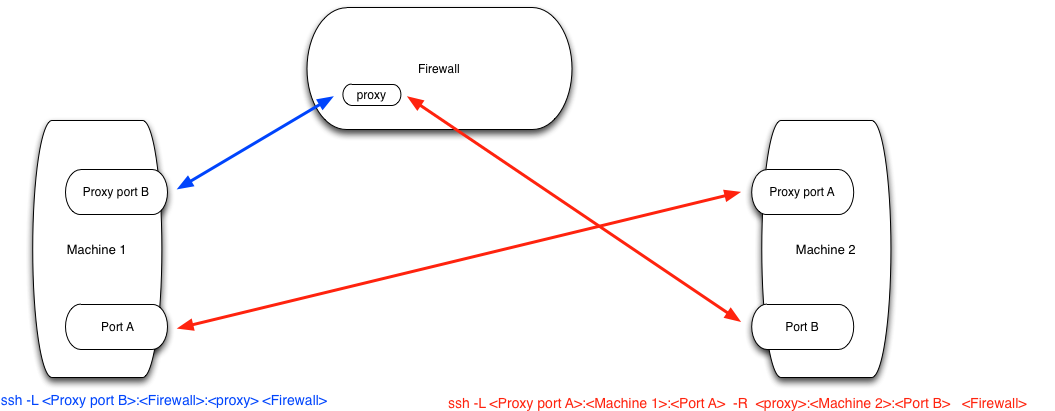
\includegraphics[scale=.30]{images/sshTunnel}
\caption{Ssh Tunnel Scenario}\label{fig:sshtunnel}
\end{center}
\end{figure}

Assuming that we have ETB servers running on these two connected machines
we can connect them by either the 
\begin{verbatim}
etb shell on machine2> tunnel("Proxy port A", "Proxy port B")
\end{verbatim}
or symmetrically 
\begin{verbatim}
etb shell on machine1> tunnel("Proxy port B", "Proxy port A")
\end{verbatim}

the situtaion that results in either case is indicated in the picture \ref{fig:2waytunnel}

\begin{figure}
\begin{center}
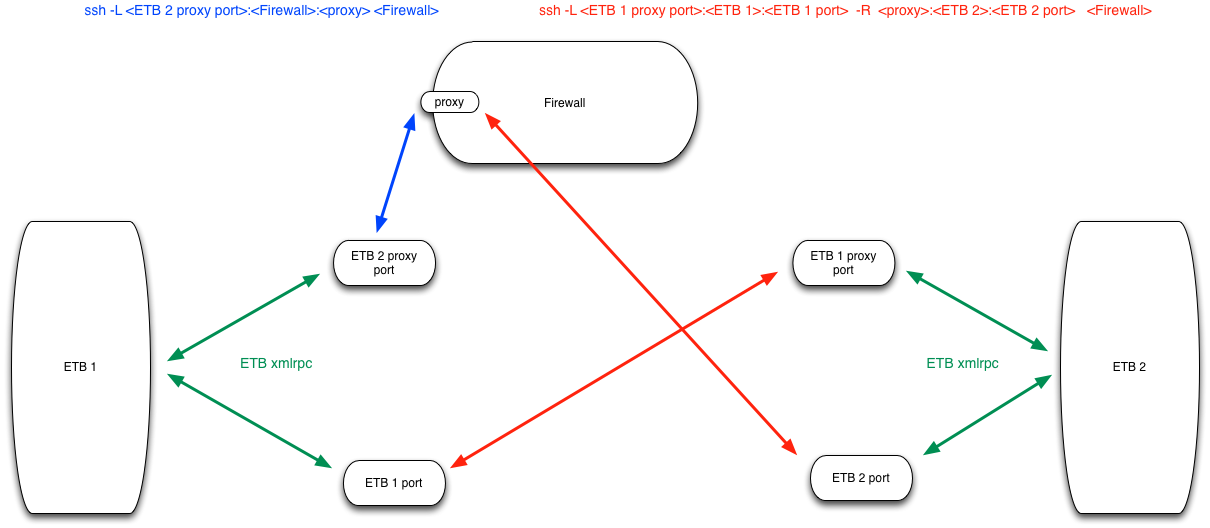
\includegraphics[scale=.30]{images/2waytunnel}
\caption{The Two Way Tunnel Scenario}\label{fig:2waytunnel}
\end{center}
\end{figure}

\subsection{The {\tt tunnel} Method}


An ETB server exposes a {\tt link} XML-RPC method:
\begin{verbatim}
tunnel(localport, remoteport)
\end{verbatim}
The arguments {\tt localport} and {\tt remoteport} correspond to 
the local proxy port on the network executing the  {\tt tunnel}
command, and the remote proxy port on the remote network.


\subsection{A {\tt tunnel} Use Case}

In order to make things more concrete, lets give a detailed 
example of doing a distributed make on two ETB networks
separated by a firewall, but connected by a tunnel.

In particular we will link a network running on a Macbook pro
{\tt pepper} with a Linux server {\tt iandev} running in SRI's cloud. 
The Macbook pro will be behind the CSL's firewall {\tt thor.csl.sri.com}.


So to begin with we start ETB servers on both machines, to make thing easier to
keep clear in our head, ports with {\tt 6}s in them will be on the Macbook,
while ports with {\tt 7}s in them will be on the Linux server. The sole
port on {\tt thor.csl.sri.com} that enters the fray will have {\tt 5}s in it.

The {\tt start} script in the {\tt demos/make} directory will accept
a port argument and start an ETB server running on that port, (and if the port is specified, 
the server will start in debug mode), otherwise it will use the default port specified
in the {\tt etb\_conf.ini} file.
\begin{verbatim}
pepper>cd etb/dmoes/make
pepper>./start 8666
...
\end{verbatim}
and 
\begin{verbatim}
iandev>cd etb/demos/make
iandev>./start 8777
...
\end{verbatim}
Now in order to connect these two networks, we first need to setup a two way {\tt ssh}
tunnel, firstly on {\tt iandev}:

\begin{verbatim}
ssh -v -L 2777:pepper:8666 -R 2555:iandev:8777  thor.csl.sri.com -N
\end{verbatim}
and secondly on {\tt pepper}:

\begin{verbatim}
ssh -v -L 2666:thor.csl.sri.com:2555  thor.csl.sri.com -N
\end{verbatim}

At this point we can test our connectivity simply using python's
command line, for example on pepper we could do:

\begin{verbatim}
import xmlrpclib
server = xmlrpclib.Server("http://localhost:2666")
server.system.listMethods()
server.get_id()
\end{verbatim}

which should return the id of the server running on {\tt iandev}, similarly 
we could do the reverse on {\tt iandev}, simply by using the 
URI {\tt "http://localhost:2777"}.

Now assuming that the above went smoothly, we can run an {\tt etb-shell}
on {\tt pepper}, and connect the two networks:
\begin{verbatim}
pepper>cd etb/demos/make
pepper>../../etb_clients/etb-shell/etb-shell -p 8666
/ > tunnel(2666, 2777)
\end{verbatim}
we could now do a compile on {\tt iandev} by doing:
\begin{verbatim}
# We first put all of our files on pepper
h1 = put_file(component1.h)
src1 = put_file(component1.c)
h2 = put_file(component2.h)
src2 = put_file(component2.c)
srcMain = put_file(main.c)
# Build everything, wait, then get the exe back
q = main("Linux_x86_64", src1, h1, src2, h2, srcMain, "main_Linux_x86_64", Exe)
r = query_wait(q)
get_file(r.Exe, "main_Linux_x86_64")
\end{verbatim}
once this has finished successfully we could do a similar feat on {\tt iandev}:
\begin{verbatim}
iandev>cd etb/demos/make
iandev>../../etb_clients/etb-shell/etb-shell -p 8777
\end{verbatim}
Note that it is not necessary to do the tunnel on this side, since the effect is
symmetric. Before we try and compile on the remote Macbook, first observe
that while the necessary files have been copied over to the linux server,
we have no way of referring to them, and thus no way to ask for the compilation to take place.

So to begin with we ask for handles to the existing files in the servers git repository,
using the the {\tt get\_filehandle} command:
\begin{verbatim}
h1 = get_filehandle(component1.h)
src1 = get_filehandle(component1.c)
h2 = get_filehandle(component2.h)
src2 = get_filehandle(component2.c)
srcMain = get_filehandle(main.c)
\end{verbatim}
We can now ask the appropriate query:
\begin{verbatim}
q = main("Darwin_i386", src1, h1, src2, h2, srcMain, "main_Darwin_i386", Exe)
\end{verbatim}




\end{document}
